\documentclass[11pt]{article}
\usepackage[a4paper,margin=25mm]{geometry}
\usepackage{booktabs}
\usepackage{graphicx}
\usepackage{amsmath,amssymb}
\usepackage{microtype}
\usepackage{xcolor}
\usepackage{siunitx}
\usepackage{array}
\usepackage{longtable}
\usepackage{subcaption}
\usepackage{float}
\usepackage[hidelinks]{hyperref}
\usepackage[numbers,sort&compress]{natbib}

\graphicspath{{figures/}}
\sisetup{round-mode=places,round-precision=3,detect-weight=true}
\newcommand{\method}[1]{\textsc{#1}}
\newcommand{\todoresult}{\textcolor{red}{[generated after the complete aligned run]}}

\title{Robust Link Prediction with Common Neighbors, GCN, and SGDiff}
\author{Jiawei Li}
\date{November 2026}

\begin{document}
\maketitle

\begin{abstract}
This report documents the Part~2 reproduction and robustness study for three
complementary link predictors: the parameter-free Common Neighbors heuristic,
a two-layer Graph Convolutional Network with a dot-product decoder, and SGDiff,
a subgraph diffusion model with structure and attribute streams. We evaluate
all methods on Cora, CiteSeer, and PubMed under one fixed team protocol. The
protocol uses identical edge splits, test pairs, attacked graphs, and metrics
for every model, and includes clean evaluation, three structural attacks at
three budgets, three additional 50\% structural perturbations, and a node
feature permutation. Component ablations isolate neighborhood aggregation,
node attributes, and SGDiff's two diffusion streams. The final numerical
summary and figures are generated directly from the audited result table.
\end{abstract}

\section{Problem and scope}
Given an undirected attributed graph $G=(V,E,X)$ and a candidate node pair
$(u,v)\notin E_{\mathrm{obs}}$, link prediction estimates whether the pair is a
held-out positive edge. Citation networks make the two main sources of
evidence especially clear. Structural methods use paths and shared
neighborhoods in $E_{\mathrm{obs}}$, while representation models can also use
the bag-of-words attributes in $X$. A robustness experiment asks how much of
this predictive signal survives when an adversary or missing-data mechanism
changes the visible graph at test time.

Our study addresses three questions. First, how do a local heuristic, a
message-passing encoder, and a conditional diffusion model compare under the
same clean link-prediction protocol? Second, which model degrades least under
random, label-aware, surrogate-guided, and one-sided structural perturbations?
Third, which input or SGDiff stream explains the observed behavior? The scope
is an evasion study: all trainable models fit the clean training graph once,
then keep their weights fixed while the evaluator changes the visible test
graph.

\section{Models and related work}
\subsection{Common Neighbors}
Common Neighbors (CN) assigns
\begin{equation}
  s_{\mathrm{CN}}(u,v)=|\Gamma(u)\cap\Gamma(v)|,
\end{equation}
where $\Gamma(u)$ is the observed one-hop neighborhood of $u$. CN is one of
the classical proximity scores studied in the link-prediction literature
\citep{libennowell2007link}. It has no learned parameters and provides a
transparent structural baseline. Its main limitation is equally transparent:
all pairs without an observed common neighbor receive the same score. NCNC
extends this principle with learned pair representations and completion of
unobserved common neighbors \citep{wang2024ncnc}; this makes the CN result a
useful mechanism-level reference for the team's NCNC study.

\subsection{GCN with a dot-product decoder}
The GCN baseline applies two normalized neighborhood-aggregation layers
\citep{kipf2017gcn} and scores a pair through the inner product of its endpoint
embeddings,
\begin{align}
  H^{(\ell+1)} &= \sigma\!\left(\widetilde D^{-1/2}
  \widetilde A\widetilde D^{-1/2}H^{(\ell)}W^{(\ell)}\right),\\
  s_{\mathrm{GCN}}(u,v) &= z_u^\top z_v.
\end{align}
This encoder-decoder pattern follows graph auto-encoder link prediction
\citep{kipf2016vgae}. Our implementation uses width 64 in both layers and
dropout 0.5. It is deliberately simpler than recent link-specific GNNs, so it
tests whether generic message passing already provides a stable neural
baseline.

Two independently trained ablations isolate its inputs. \method{GCN-no-neighbors}
replaces message passing with a width-matched MLP, preserving attributes and
capacity while removing graph aggregation. \method{GCN-no-attributes}
replaces every node feature row with the same constant vector, preserving the
graph and message passing while removing attribute identity.

\subsection{SGDiff}
SGDiff extracts a local enclosing subgraph for each candidate pair and models
the evidence under the edge and non-edge hypotheses with conditional diffusion
\citep{li2025sgdiff}. Its structure stream denoises discrete structural labels;
its feature stream denoises node attributes with a GCN; a learned Bayesian
fusion module combines the two class-conditional scores. This design differs
from a discriminative GCN because it asks how well each candidate hypothesis
explains the observed local subgraph rather than directly mapping endpoint
embeddings to a link probability.

We report three readouts from one trained checkpoint: full fusion,
structure-only, and feature-only. The single-stream readouts reuse exactly the
same extracted subgraphs, diffusion draws, and learned model. They therefore
measure how much evidence each trained stream contributes at test time; they
are not separately retrained single-stream models.

\section{Experimental design}
\subsection{Data and splits}
We use the standard Planetoid versions of Cora, CiteSeer, and PubMed
\citep{yang2016planetoid}. For each dataset and seed $s\in\{0,1,2\}$, existing
undirected edges are split into 80\% training, 5\% validation, and 15\% test
positives. Each split receives an equal number of sampled non-edges, and the
negative sets are mutually disjoint. Model fitting sees only training
positives as graph edges. Test-time context contains the training and
validation positive edges, while validation and test candidates remain
protected from attack insertion.

The run verifies every split array against the team's published split files.
It also verifies a SHA-256 fingerprint for every attacked graph. A mismatch
terminates the run rather than producing a nominally comparable row.

\subsection{Training}
CN requires no fitting. Each GCN configuration trains independently on CUDA
with Adam, learning rate $10^{-2}$, at most 100 epochs, validation every five
epochs, and patience 30. The selected checkpoint minimizes validation loss.

SGDiff uses the dataset-specific Table~4 architecture and diffusion steps from
the original work: one-hop enclosing subgraphs; no per-hop cap for Cora and a
20-node cap for CiteSeer and PubMed; structural diffusion lengths 20, 20, and
10; and feature diffusion lengths 100, 100, and 50. Training uses the complete
training split, batch size 32, and all diffusion timesteps rather than a
Monte-Carlo subset. Diffusion pretraining runs for at most 50 epochs with
validation early stopping. The frozen-diffusion fusion stage runs for five
epochs and selects the minimum validation loss. The paper does not state an
epoch count for this stage; consequently, these results should be described as
a full-data team-benchmark reproduction with a declared five-epoch fusion
budget, not as a bitwise reproduction of a historical 20-epoch run.

All trainable models run on an NVIDIA GeForce RTX 3060 Laptop GPU with 6~GiB
memory, PyTorch 2.5.1+cu121, and CUDA 12.1. The Cora and CiteSeer EA graphs are
the pinned CUDA assets from the team evaluator. PubMed EA generation exceeds
local memory, so the experiment reads the team's published H200 graph assets
rather than regenerating a different attack locally. This affects attack
generation hardware, not the graph presented to each predictor.

\subsection{Robustness conditions}
Each seed has 14 test conditions:
\begin{enumerate}
  \item clean evaluation;
  \item random edge flips (RF) at 10\%, 25\%, and 50\%;
  \item DICE at 10\%, 25\%, and 50\%, deleting same-class edges and inserting
        different-class edges \citep{waniek2018hiding};
  \item a surrogate-guided embedding attack (EA) at 10\%, 25\%, and 50\%,
        following the graph-attack setting of \citet{zugner2019meta};
  \item random deletion, hub-priority deletion, and random insertion, each at
        50\%;
  \item a row-wise permutation of node attributes with graph edges unchanged.
\end{enumerate}
For RF, DICE, and EA, the percentage denotes the total edge-edit budget, with
deletions and insertions sharing that budget. The class labels used by DICE
are privileged attacker information and are never provided to a predictor.
The EA graphs are fixed team assets generated once with the pinned surrogate,
so every model receives exactly the same attacked graph.

\subsection{Metrics and fairness controls}
We report AUROC, average precision (AP), Hits@100, and Precision@100. Hits@100
follows the ranking-oriented convention used in graph link-prediction
benchmarks \citep{hu2020ogb}. AUROC and AP are the primary global ranking
metrics; the top-100 metrics expose whether a method concentrates positives at
the top of the candidate list.

Fair comparison here means identical data and evaluation, not identical
floating-point operation counts. All methods use the same split, complete
test candidate set, visible graph, perturbation asset, metric implementation,
and three seeds. Each trainable method retains a reasonable method-specific
optimizer and training recipe. This choice compares trained predictors under
one task protocol; it is not an equal-compute study.

\section{Results}
\label{sec:results}
\IfFileExists{generated/results_tables.tex}{\subsection{Clean link prediction}
Table~\ref{tab:clean} reports all four clean metrics. Values are mean $\pm$ sample standard deviation over three seeds.
\begin{table}[H]
\centering
\small
\begin{tabular}{llcccc}
\toprule
Dataset & Model & AUROC & AP & Hits@100 & Precision@100 \\
\midrule
Cora & CN & 0.722 $\pm$ 0.004 & 0.720 $\pm$ 0.004 & 0.452 $\pm$ 0.006 & 1.000 $\pm$ 0.000 \\
Cora & GCN & 0.846 $\pm$ 0.010 & 0.860 $\pm$ 0.010 & 0.669 $\pm$ 0.012 & 0.973 $\pm$ 0.012 \\
Cora & SGDiff & 0.853 $\pm$ 0.006 & 0.854 $\pm$ 0.022 & 0.723 $\pm$ 0.018 & 0.933 $\pm$ 0.046 \\
\addlinespace
CiteSeer & CN & 0.669 $\pm$ 0.002 & 0.668 $\pm$ 0.002 & 0.340 $\pm$ 0.006 & 0.998 $\pm$ 0.002 \\
CiteSeer & GCN & 0.823 $\pm$ 0.004 & 0.841 $\pm$ 0.006 & 0.639 $\pm$ 0.015 & 0.970 $\pm$ 0.010 \\
CiteSeer & SGDiff & 0.836 $\pm$ 0.018 & 0.856 $\pm$ 0.016 & 0.689 $\pm$ 0.024 & 0.970 $\pm$ 0.017 \\
\addlinespace
PubMed & CN & 0.642 $\pm$ 0.002 & 0.642 $\pm$ 0.002 & 0.286 $\pm$ 0.004 & 1.000 $\pm$ 0.000 \\
PubMed & GCN & 0.954 $\pm$ 0.002 & 0.958 $\pm$ 0.002 & 0.616 $\pm$ 0.012 & 1.000 $\pm$ 0.000 \\
PubMed & SGDiff & 0.904 $\pm$ 0.005 & 0.900 $\pm$ 0.009 & 0.302 $\pm$ 0.047 & 0.983 $\pm$ 0.006 \\
\bottomrule
\end{tabular}
\caption{Clean performance under the aligned evaluator.}
\label{tab:clean}
\end{table}

\subsection{Strong structural perturbations}
Table~\ref{tab:strong} gives AUROC at the 50\% budgets and the change from the matched clean mean.
\begin{table}[H]
\centering
\small
\begin{tabular}{llccc}
\toprule
Dataset & Model & RF 50\% & DICE 50\% & EA 50\% \\
\midrule
Cora & CN & 0.642 (-0.080) & 0.642 (-0.080) & 0.732 (+0.010) \\
Cora & GCN & 0.804 (-0.042) & 0.796 (-0.050) & 0.837 (-0.009) \\
Cora & SGDiff & 0.768 (-0.085) & 0.754 (-0.099) & 0.800 (-0.054) \\
\addlinespace
CiteSeer & CN & 0.616 (-0.052) & 0.604 (-0.065) & 0.689 (+0.020) \\
CiteSeer & GCN & 0.794 (-0.030) & 0.794 (-0.029) & 0.802 (-0.022) \\
CiteSeer & SGDiff & 0.736 (-0.100) & 0.741 (-0.095) & 0.819 (-0.017) \\
\addlinespace
PubMed & CN & 0.601 (-0.041) & 0.600 (-0.042) & 0.657 (+0.015) \\
PubMed & GCN & 0.914 (-0.040) & 0.908 (-0.046) & 0.948 (-0.006) \\
PubMed & SGDiff & 0.856 (-0.048) & 0.855 (-0.049) & 0.893 (-0.011) \\
\bottomrule
\end{tabular}
\caption{AUROC under the strongest RF, DICE, and EA settings. Parentheses show the change from clean.}
\label{tab:strong}
\end{table}
}{\todoresult}

\IfFileExists{figures/clean_auroc.pdf}{
\begin{figure}[H]
  \centering
  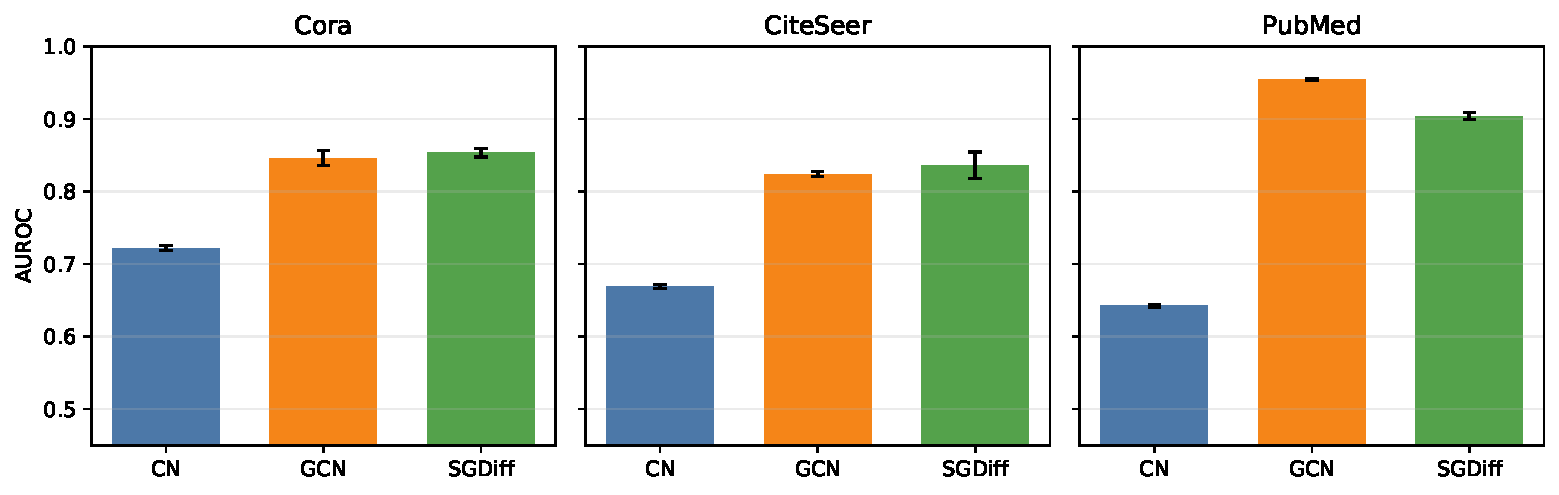
\includegraphics[width=0.92\linewidth]{clean_auroc.pdf}
  \caption{Clean AUROC, averaged over three seeds. Error bars show sample
  standard deviation.}
  \label{fig:clean}
\end{figure}}{}

\IfFileExists{figures/attack_curves.pdf}{
\begin{figure}[H]
  \centering
  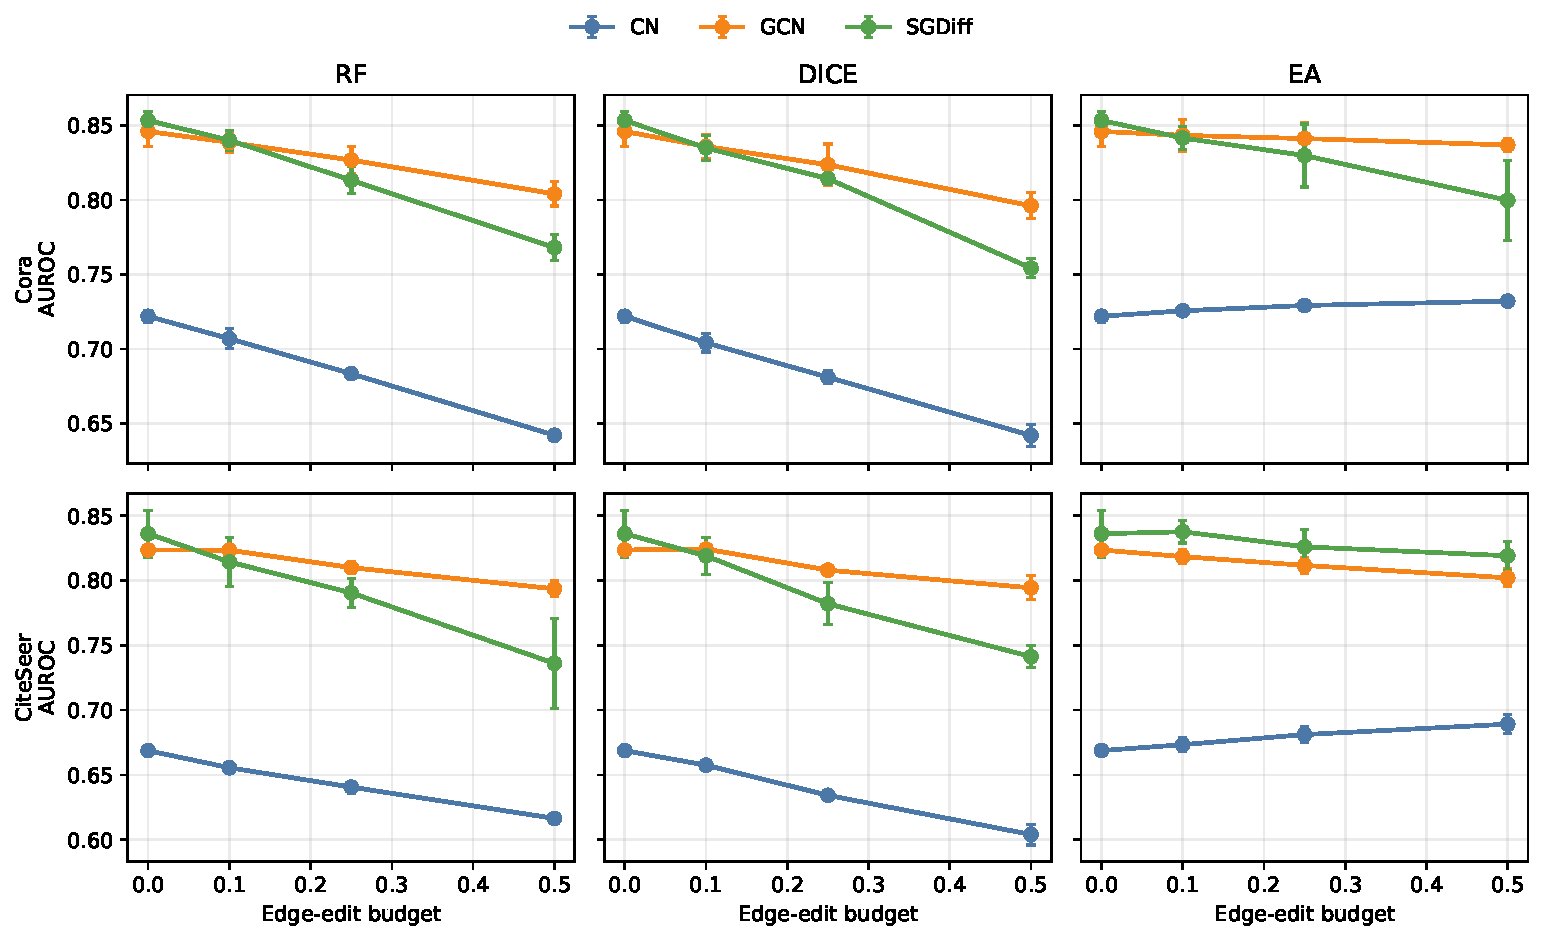
\includegraphics[width=\linewidth]{attack_curves.pdf}
  \caption{AUROC under RF, DICE, and EA. Every point uses the same attacked
  graph for all models within a dataset and seed.}
  \label{fig:attacks}
\end{figure}}{}

\IfFileExists{figures/robustness_heatmap.pdf}{
\begin{figure}[H]
  \centering
  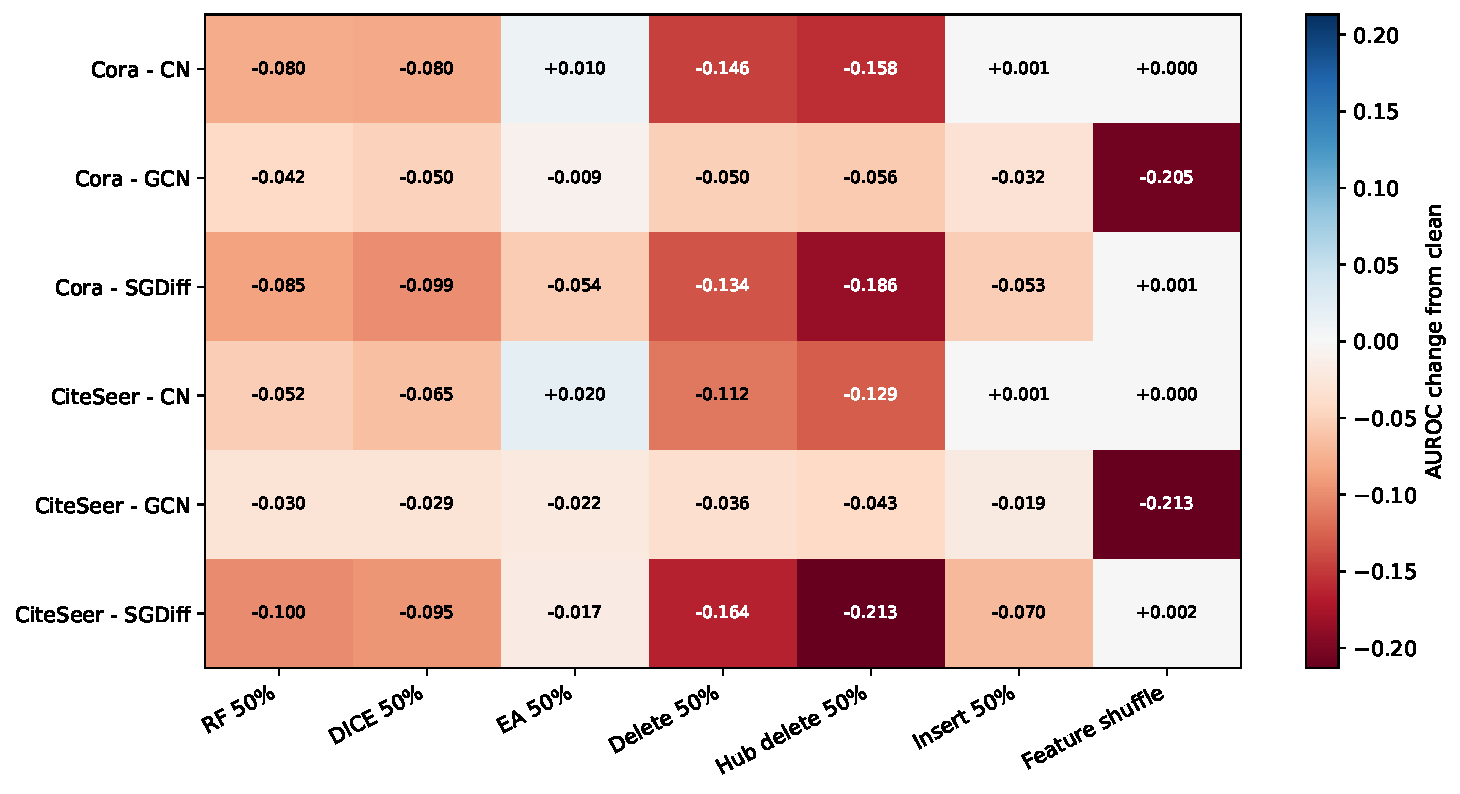
\includegraphics[width=0.98\linewidth]{robustness_heatmap.pdf}
  \caption{Change in AUROC from the matched clean result. More negative values
  indicate greater degradation.}
  \label{fig:heatmap}
\end{figure}}{}

\IfFileExists{generated/ncnc_comparison.tex}{\subsection{CN compared with the team's NCNC result}
Table~\ref{tab:cn-ncnc} uses Junxiong's full NCNC rows from the same pinned evaluator. The team reference covers Cora and CiteSeer, so PubMed is not extrapolated.
\begin{table}[H]
\centering
\resizebox{\linewidth}{!}{%
\begin{tabular}{llccccc}
\toprule
Dataset & Model & Clean & RF 50\% & DICE 50\% & EA 50\% & Feature shuffle \\
\midrule
Cora & CN & 0.722 $\pm$ 0.004 & 0.642 $\pm$ 0.004 & 0.642 $\pm$ 0.008 & 0.732 $\pm$ 0.003 & 0.722 $\pm$ 0.004 \\
Cora & NCNC & 0.959 $\pm$ 0.002 & 0.936 $\pm$ 0.006 & 0.934 $\pm$ 0.006 & 0.944 $\pm$ 0.003 & 0.692 $\pm$ 0.017 \\
\addlinespace
CiteSeer & CN & 0.669 $\pm$ 0.002 & 0.616 $\pm$ 0.004 & 0.604 $\pm$ 0.008 & 0.689 $\pm$ 0.007 & 0.669 $\pm$ 0.002 \\
CiteSeer & NCNC & 0.968 $\pm$ 0.007 & 0.950 $\pm$ 0.003 & 0.945 $\pm$ 0.002 & 0.950 $\pm$ 0.006 & 0.637 $\pm$ 0.037 \\
\bottomrule
\end{tabular}
}%
\caption{AUROC for parameter-free CN and the team's learned NCNC model under matched data and perturbations.}
\label{tab:cn-ncnc}
\end{table}
NCNC is substantially stronger on the clean graph and under structural edits. Feature shuffling removes much of that advantage because NCNC uses learned node representations, whereas CN ignores attributes and therefore reproduces its clean score exactly. This does not make CN the stronger overall predictor; it identifies the source of its invariance.
}{}

\subsection{Performance around high-degree nodes}

Following the team's degree-stratified diagnostic, we rank nodes by degree in each seed's clean training graph. For a given $k$, we select the top $k\%$ nodes, breaking degree ties by node ID, and evaluate the original held-out test pairs with at least one endpoint in that set. The node set and test pairs remain fixed across all models and perturbations. We use $k\in\{1,5,10,20,50,100\}$, and report AUROC and AP only when the selected cohort contains both classes. All 14 conditions, seven model variants, and three seeds are retained in the accompanying CSV files; the main plots show clean and 50\% hub-priority edge deletion.

\begin{table}[H]

\centering

\small

\begin{tabular}{llccc}

\toprule

Dataset & Model & Top 5\% & Top 20\% & All nodes \\

\midrule

Cora & CN & 0.751 & 0.751 & 0.722 \\

Cora & GCN & 0.830 & 0.854 & 0.846 \\

Cora & SGDiff & 0.803 & 0.853 & 0.853 \\

\midrule

Citeseer & CN & 0.741 & 0.723 & 0.669 \\

Citeseer & GCN & 0.854 & 0.843 & 0.823 \\

Citeseer & SGDiff & 0.858 & 0.863 & 0.836 \\

\midrule

Pubmed & CN & 0.692 & 0.650 & 0.642 \\

Pubmed & GCN & 0.947 & 0.945 & 0.954 \\

Pubmed & SGDiff & 0.795 & 0.828 & 0.904 \\

\bottomrule

\end{tabular}

\caption{Clean AUROC on test pairs incident to nodes with the highest clean training degree. Values average three seeds. The 100\% column is the original full-test AUROC.}

\label{tab:topdegree}

\end{table}

\begin{figure}[H]

\centering

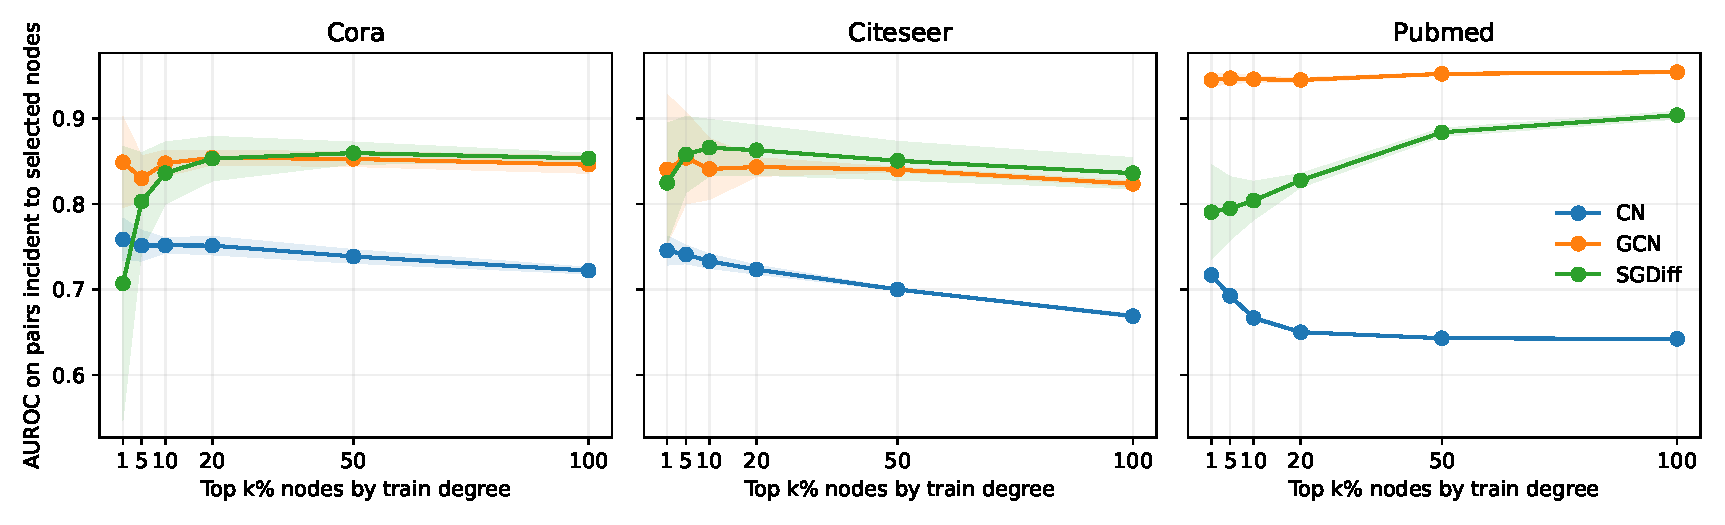
\includegraphics[width=\linewidth]{clean_top_degree_auc.pdf}

\caption{Clean AUROC as the high-degree node cohort expands. Shading shows standard deviation across three seeds.}

\label{fig:topdegreeclean}

\end{figure}

\begin{figure}[H]

\centering

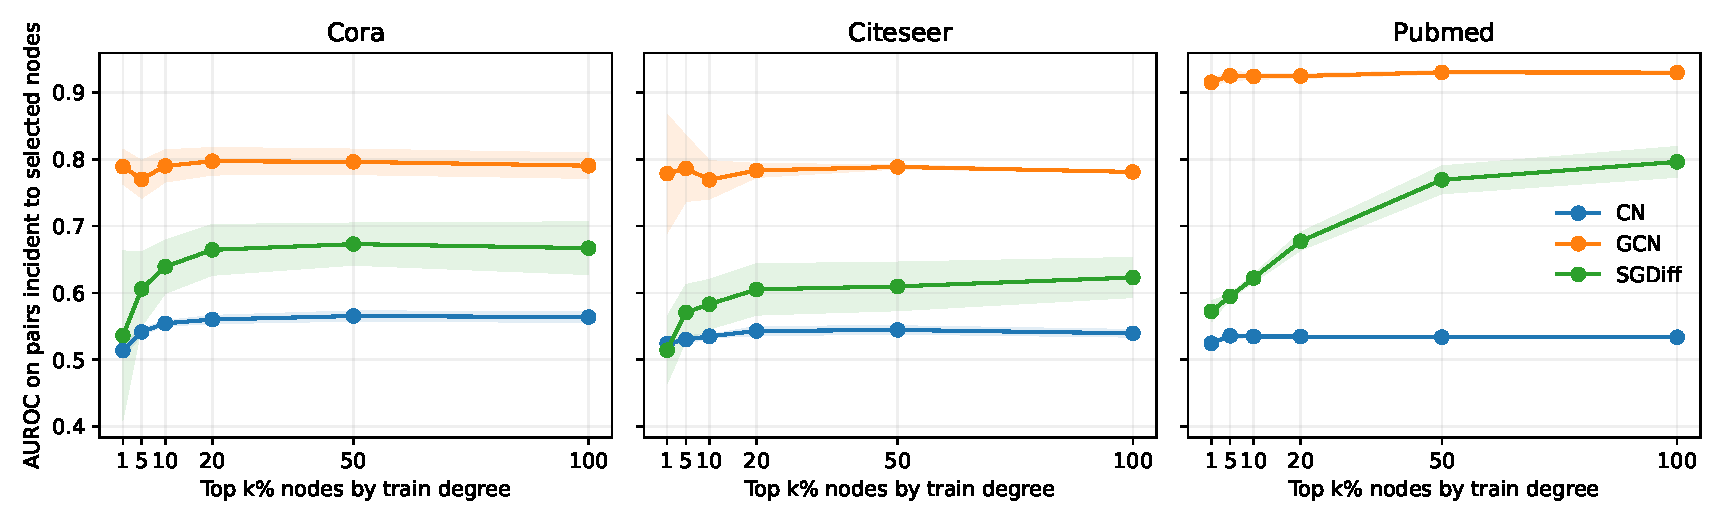
\includegraphics[width=\linewidth]{hub_delete_50_top_degree_auc.pdf}

\caption{The same fixed cohorts under 50\% hub-priority edge deletion.}

\label{fig:topdegreehubdelete}

\end{figure}

The top 1\% cohorts are highly imbalanced, especially in Cora and CiteSeer, and their curves vary substantially across seeds. Cohort AUROC is conditional on node degree; it is not the precision of the model's highest-scoring predicted links. These observations alone do not establish that SGDiff's subgraph node cap causes its hub behavior.


\section{Component ablations}
\label{sec:ablations}
\IfFileExists{generated/ablation_text.tex}{\subsection{GCN inputs}
For Cora, removing neighbor aggregation changes clean AUROC by -0.062, while removing node attributes changes it by -0.170.
For CiteSeer, removing neighbor aggregation changes clean AUROC by -0.037, while removing node attributes changes it by -0.180.

\subsection{SGDiff streams}
For Cora, the stronger single SGDiff readout is structure-only (0.808 AUROC), compared with 0.853 for learned fusion.
For CiteSeer, the stronger single SGDiff readout is structure-only (0.824 AUROC), compared with 0.836 for learned fusion.
These readouts share one trained checkpoint and one set of diffusion evidence. They identify which stream the fitted model uses at test time; they do not estimate the performance of independently retrained single-stream models.
}{\todoresult}

\IfFileExists{figures/ablations.pdf}{
\begin{figure}[H]
  \centering
  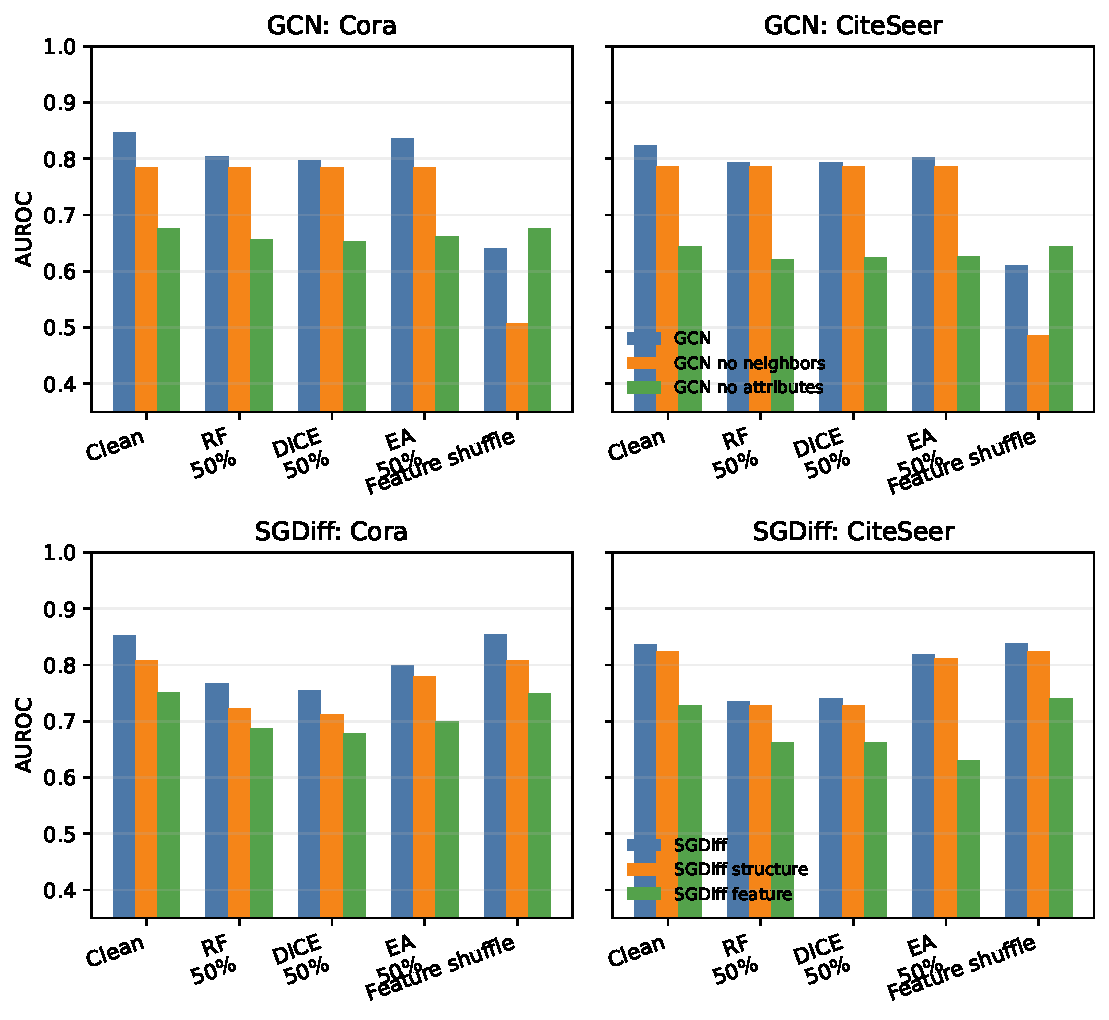
\includegraphics[width=\linewidth]{ablations.pdf}
  \caption{Clean and perturbed AUROC for the GCN input ablations and SGDiff
  stream readouts.}
  \label{fig:ablations}
\end{figure}}{}

\section{Discussion and limitations}
\IfFileExists{generated/discussion.tex}{\subsection{Main comparison}
On Cora, SGDiff has the highest clean AUROC among the three primary models (0.853). On CiteSeer, SGDiff has the highest clean AUROC among the three primary models (0.836).

\subsection{Robustness}
Across the 13 perturbed conditions on Cora, SGDiff has the highest worst-case AUROC (0.667). Across the 13 perturbed conditions on CiteSeer, SGDiff has the highest worst-case AUROC (0.623).
Figure~\ref{fig:attacks} separates attack budget from attack type, while Figure~\ref{fig:heatmap} reports matched clean-to-attack changes. Absolute attacked AUROC and degradation should be read together: a low-capacity model can show a small drop simply because its clean score is already low.
}{\todoresult}

The study has four interpretation limits. First, three random seeds quantify
large run-to-run changes but do not support fine-grained significance claims.
Second, all attacks are evasion conditions; adversarial retraining could change
the ranking. Third, the local EA implementation uses the team's fixed linear
surrogate and is not guaranteed to reproduce an unreleased author attack.
Fourth, SGDiff and CN/GCN use different method-appropriate training budgets,
so the study should not be presented as an efficiency-normalized comparison.

\bibliographystyle{plainnat}
\bibliography{references}
\end{document}
